\documentclass[border=4pt]{standalone}
\usepackage{amsmath,amssymb}
\usepackage{tikz}
\usetikzlibrary{positioning,arrows.meta}
\definecolor{cblue}{HTML}{2a78d6}
\definecolor{corange}{HTML}{eb6834}
\definecolor{cgray}{HTML}{8a8983}
\begin{document}
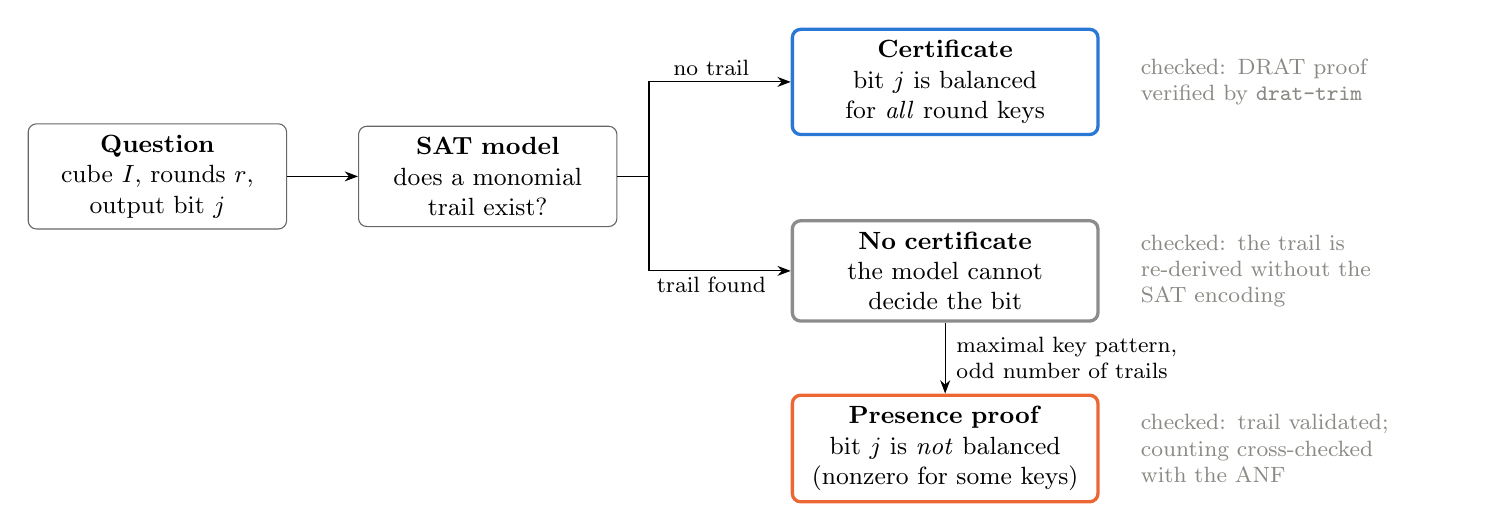
\begin{tikzpicture}[font=\small, >=Stealth, node distance=5mm and 9mm,
  box/.style={draw=black!60, rounded corners=3pt, align=center, inner sep=4pt, minimum height=11mm},
  res/.style={box, very thick, text width=36mm},
  chk/.style={align=left, font=\footnotesize, text=cgray, text width=40mm},
  lab/.style={font=\footnotesize, fill=white, inner sep=1pt}]
\node[box, text width=30mm] (q) {\textbf{Question}\\ cube $I$, rounds $r$,\\ output bit $j$};
\node[box, text width=30mm, right=of q] (sat) {\textbf{SAT model}\\ does a monomial\\ trail exist?};
\node[res, draw=cblue, right=22mm of sat, yshift=12mm] (cert) {\textbf{Certificate}\\ bit $j$ is balanced\\ for \emph{all} round keys};
\node[res, draw=black!45, right=22mm of sat, yshift=-12mm] (maybe) {\textbf{No certificate}\\ the model cannot\\ decide the bit};
\node[res, draw=corange, below=9mm of maybe] (pres) {\textbf{Presence proof}\\ bit $j$ is \emph{not} balanced\\ (nonzero for some keys)};
\node[chk, right=4mm of cert] {checked: DRAT proof\\ verified by \texttt{drat-trim}};
\node[chk, right=4mm of maybe] {checked: the trail is\\ re-derived without the\\ SAT encoding};
\node[chk, right=4mm of pres] {checked: trail validated;\\ counting cross-checked\\ with the ANF};
\draw[->] (q) -- (sat);
\coordinate (fork) at ([xshift=4mm]sat.east);
\draw (sat.east) -- (fork);
\draw[->] (fork) |- (cert.west) node[lab, pos=0.72, above=1pt] {no trail};
\draw[->] (fork) |- (maybe.west) node[lab, pos=0.72, below=1pt] {trail found};
\draw[->] (maybe.south) -- node[lab, right, align=left, xshift=1mm] {maximal key pattern,\\ odd number of trails} (pres.north);
\end{tikzpicture}
\end{document}
